\chapter{Market Analysis}
\label{ch:Market_Analysis}
Analysing and understanding the Urban Air Mobility (UAM) market in \Cref{sec:UAM_Market} lays the foundation for the market entrance of the \textit{Swing eVTOL}.
After which, the deeper dive into the market segmentation in \Cref{sec:Market_Segmentation}, in use cases and geographical locations, can point out the most interesting part of the market.
The infrastructure, regulations and even attractive partnerships come with the market segmentation, which is discussed in \Cref{sec:Vertiports,sec:UKAM_Consortium}.
Furthermore, the competition analysis in \Cref{sec:Competition_Analysis} provides more market context, paving the way for the differentiation factor of the \textit{Swing eVTOL}.

\section{UAM Market}
\label{sec:UAM_Market}
The UAM market covers the new ways of transport in the third dimension, using the latest technologies in the eVTOL industry, which is hence of interest to this project.
Although relatively new, it can be considered a very promising market.
An in-depth market analysis performed by Roland Berger consultancy deems the UAM market to have great potential; by 2050, it could become a 90 billion USD market with \num[exponent-mode=input]{160000} commercial UAM vehicles in use~\cite{potential90uam}.
While currently at the beginning of its market maturity, it is valued at not even one billion USD, thus suitable for the market penetration of this transwing eVTOL design~\cite{SAMUAM}.
The total UAM market consists of at least the following applications: air taxis, airport shuttles, interurban transport, last-mile transport, air metro, private transport, military services, air emergency services, mapping, surveillance, and many more.
Hence, various applications are suitable for the \textit{Swing eVTOL}; however, those are discussed later in market segmentation (\Cref{sec:Market_Segmentation}).
Another recent market analysis on UAM that focused more on the air taxi applications, thus point-to-point passenger services, found that air taxis would replace non-discretionary travel of more than 45 min~\cite{goyal2021advanced}.
Therefore, concluding a daily demand of \num[exponent-mode=input]{82000} passengers in the US\ only right now, hence around 4000 flight hours for a four-seater eVTOL like the \textit{Swing eVTOL}.
The market study also states that in the most conservative estimation, the air taxi market would already account for 2.5 billion USD\@.
Therefore, this design is expected to be most successful in the air taxi segment, as the UAM market is highly dependent on its demand \cite{long2023demand}, confirmed by the previously discussed paper.

\subsection*{Stakeholders}
\begin{minipage}{0.4\linewidth}
    Considering the UAM market, a distinction can be made between the four main stakeholder entities: lawmakers, users, suppliers, and other involved parties.
    More detailed stakeholders can be retrieved from these four, together with their interest and influence on this project.
    After an elaborate stakeholder analysis, which entailed identification and interest/influence estimation, the following stakeholder map is established in \Cref{fig:stakeholders_analysis}.
    In particular, the investors, UAM operator prospects, Delft University of Technology, partnerships, maintenance contractors, vertiport operators, passengers, manufacturers, and air and ground regulatory agencies should be managed closely, as these significantly influence this project.
    Clear communication with these key stakeholders is important in conducting a successful project.
\end{minipage}
\begin{minipage}{0.6\linewidth}
    \begin{figure}[H]
        \centering
        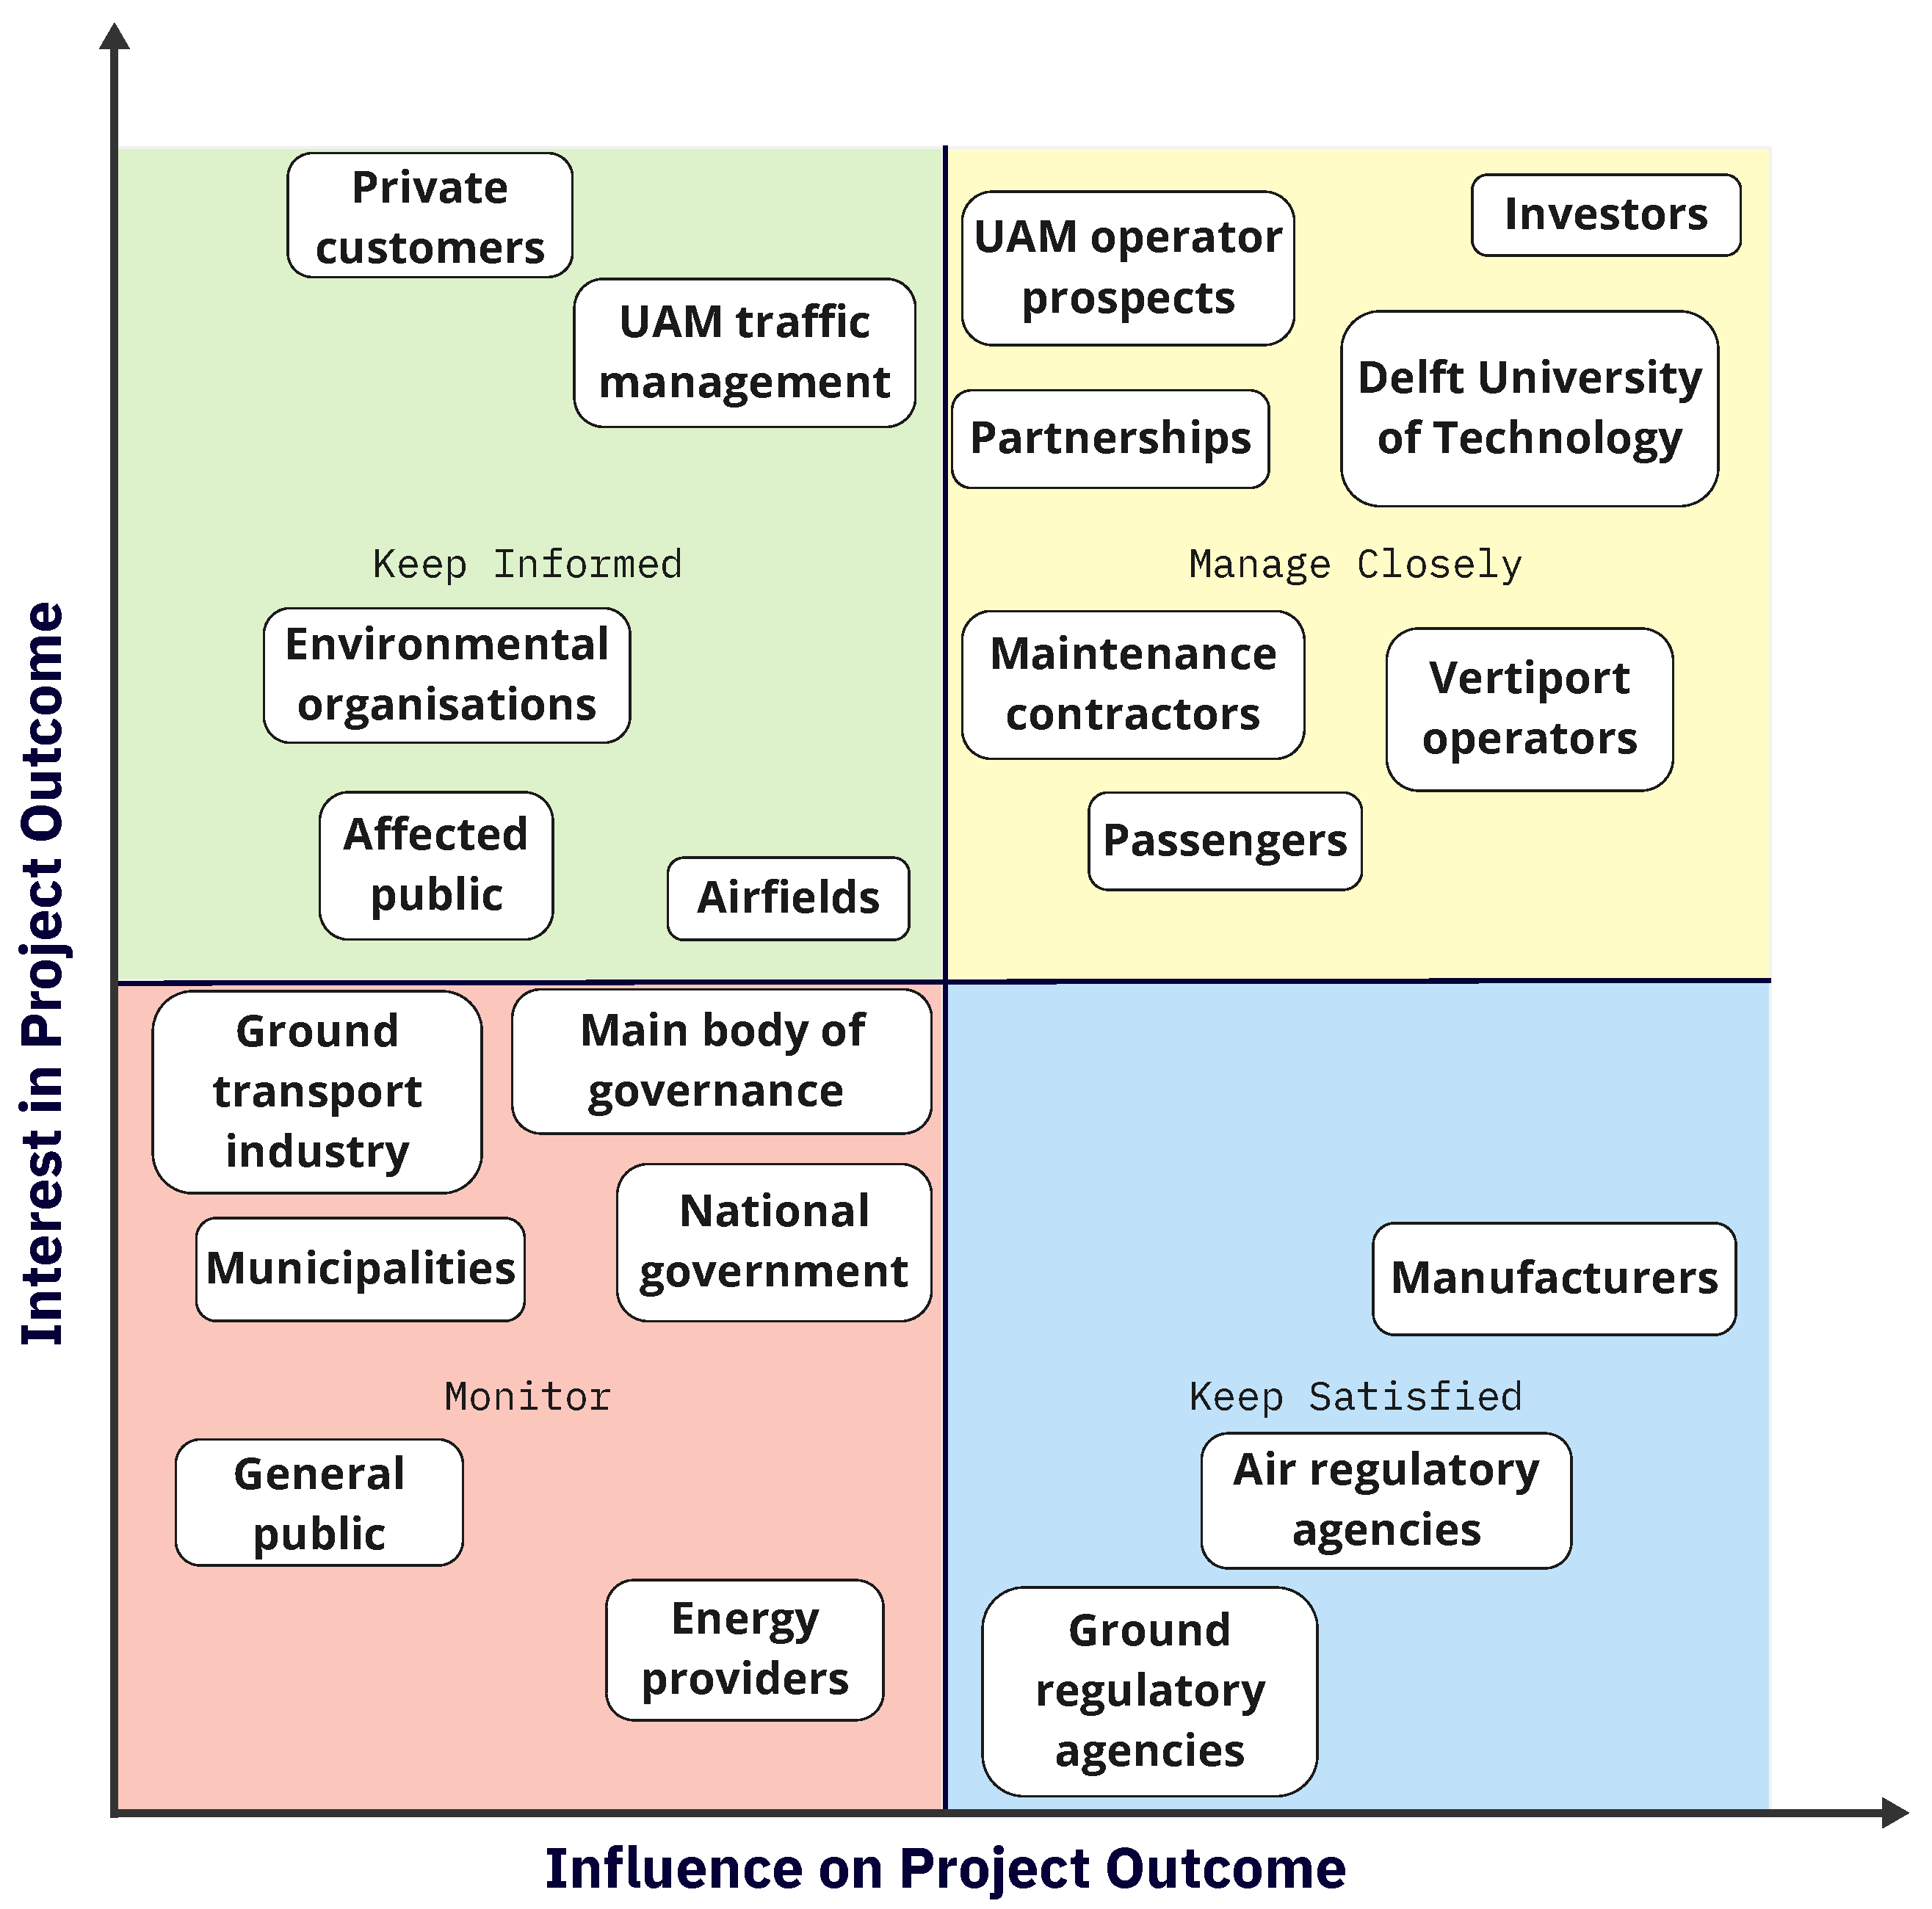
\includegraphics[width=0.9\linewidth]{figures/Stakeholder Analysis (1)}
        \caption{Stakeholder analysis}
        \label{fig:stakeholders_analysis}
    \end{figure}
\end{minipage}


\section{Market Segmentation}
\label{sec:Market_Segmentation}
To successfully analyse the suitable market for this design, proper market segmentation needs to be conducted to fully grasp the design's possibilities.
From the earlier stated applications, the main focus areas are on three leading use cases: air taxi, airport shuttle, and interurban transport \cite{UAMroland}.
Moreover, this is further solidified by the discussed 2.5 billion USD air taxi market that is currently possible \cite{goyal2021advanced}.
A fourth and very specific use case is last-mile transport, which provides transportation to the exact final destination, where the design of the \textit{Swing eVTOL} comes to fruition.
Due to the novel transformative wing design, it can account for all these four cases, as it has a great range while still having a low ground footprint.
However, this application's (competitive) advantage will be further discussed in \Cref{sec:differentiation_factor}.
It should be noted that the \textit{Swing eVTOL} can be compatible in other use cases as well, but for the first stages, these are the focus areas, hence the chosen market segment.

Before choosing a geographical market segment that fits the use cases, it is helpful to describe each in greater detail for clarification.
Urban taxis, with a range of 15 to 50 km \cite{potential90uam}, account for fast travel times as well as high coverage in urban environments.
Hence, needing a broad network of take-off and landing facilities, also known as vertiports and a closely managed UAM traffic control.
Airport shuttles, also with a range of 15 to 50 km, establish a much faster airport-to-city, and vice versa, as well as an airport-to-airport network.
This would greatly improve transfer times, transportation efficiency, and the experience that comes with airport travel.
Interurban transport, with a range of 50 to 250 km, provides a high-speed option for further travel without needing lots of infrastructure while having a relatively predictable demand \cite{UAMroland}.
The fact that the \textit{Swing eVTOL} can cover both inter-and urban transport due to its greater range for low ground footprint eVTOLs differentiates it from the current market.
Lastly, the last-mile transport, or transport, can be in combination with any of the three use cases, hence delivering the option other current eVTOLs cannot satisfy.

\subsection*{Geographical}
To thoroughly analyse and choose the market segment, a linked geographic location will benefit the team greatly in terms of the eventual regulations, partnerships, infrastructure, and competition.
This also further defines the project's requirements, constraints, and risks.
The metropolitan areas in continental Europe have been thoroughly analysed due to innovation, sustainably, and financially driven societies in combination with densely populated areas desperate for a solution.
The most interesting candidates concluded Paris (urban transport), The Randstad (interurban transport), and London (inter- and urban transport).
Eventually, London was the most attractive geographical market for the \textit{Swing eVTOL} because of its densely populated city centre and surrounding cities that conclude the so-called \enquote*{London borough}.
Therefore, making up for a combination of a vast urban environment that also accounts for interurban transport with its surrounding cities, tackling two of the use cases.
With the newly found range of \qty{250}{\km} in \Cref{ch:eps}, intercity flights from London to Manchester would even be possible.
The airport shuttle case is also favourable for London, as the metropolitan area has six airports: Heathrow, Gatwick, Stansted, Luton, City, and Southend, with Heathrow being the largest airport in Europe.
London is known to be rather traffic-dense, so the third dimension of transport provides the perfect solution.
To exemplify, a trip from Heathrow to the city centre of London (\qty{32}{km}) would take 60 to 90 minutes by car and 55 minutes by train.
However, with eVTOL vehicles, it would take merely 13 minutes~\cite{UKAMC2022benefits}, hence 47 to 77 minutes and 42 minutes faster than the current options, respectively.
Furthermore, as the \textit{Swing eVTOL} has a low ground footprint, the last-mile transportation is suitable in the tightly packed city of London.
More importantly, a consortium has even been established, which focuses on being the front runner of UAM on a greater scale, and will be further discussed in \Cref{sec:UKAM_Consortium}.


\section{Vertiports}
\label{sec:Vertiports}
As the infrastructure accommodating UAM is at the forefront of its technology and regulations, a deeper dive into vertiports is of great interest to the design.
EASA’s main regulatory framework states that a \enquote*{vertiport means an area of land, water, or structure used or intended to be used for the landing and take-off of VTOL-capable aircraft} (EASA SC-VTOL-01) \cite{easa2022vertiports}.
Therefore, vertiports is a collection term for the different configurations of take-off and landing sites that facilitate UAM.
They are fundamental to successfully introducing UAM, making for a more efficient means of travel.
Considering these vertiports would have to be placed as strategically as possible for their designed transport, they must also include additional infrastructure, such as fast charging stations, maintenance stations, and commercial services.
The implementation of vertiports is soon to be realised since the Olympic Games in Paris participates in the first test vertiport, accommodated by Skyports.
The apparent benefit of UAM is the time efficiency that comes with it, as a trip to the Olympic stadium will be reduced from 50 to 15 minutes \cite{rijksoverheid_vertiports}.
\subsection{Typical configurations}
These vertiports come in various configurations, personalised to their use case obviously, but also to the preferred size and position.
More so with the \textit{Swing eVTOL}, due to its low ground footprint of four parking spaces and wheel configuration, which make taxiing possible.
Therefore, vertiports can be defined into three main types; verstops, vertibases, and vertihubs, exemplified in \Cref{fig:vertiport_configs}.
The vertistop configuration consist of one Final-Approach and Take-Off area (FATO), thus the most compact type of vertiport, acting only as a stop for the delivery of the payload, hence being applicable in most population-dense areas.
\Cref{ch:Operations_and_Logistics} will elaborate further upon the eventual emergency charging systems available in such a minimal configuration.
The middle-sized vertiport would be the vertibase; which can either be placed on buildings and ground, and make up more than one FATO, some aprons, one terminal, and some extra services.
Lastly, the vertihub concludes the largest configuration, consisting of multiple FATOs, many aprons, multiple terminals, air traffic control, maintenance stations, charging stations, and commercial services.
Vertihubs would mainly be positioned at the edges of urban environment, taking up much space, or connected to airports.
Due to the novel transwing design, the \textit{Swing} would apply to all applications.

\begin{figure}[H]
    \centering
    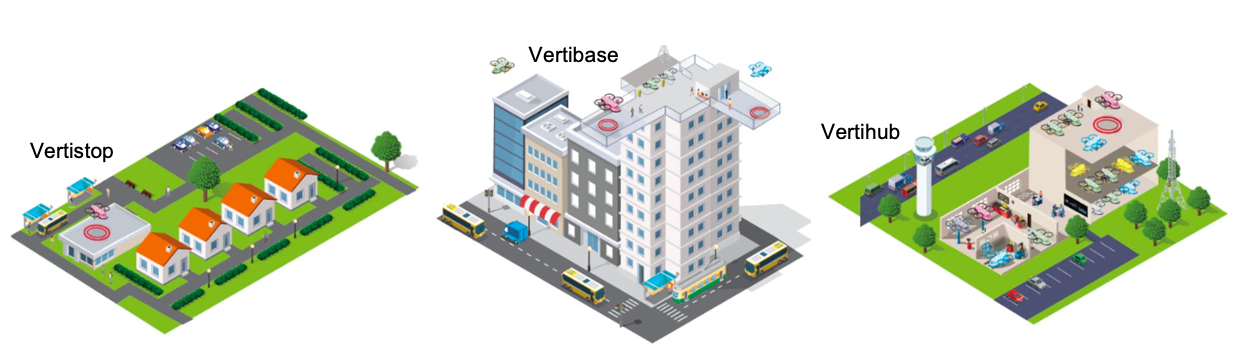
\includegraphics[width=1.0\linewidth]{figures/Market Analysis/Vertiport-configs-final.png}
    \caption{Vertiport configurations \cite{rijksoverheid_vertiports}}
    \label{fig:vertiport_configs}
\end{figure}

\subsection{Regulations}
Due to the already overly full airspace and the environmental impact that UAM will have, clear regulations regarding the vertiports are paramount.
The main body regulating UAM in Europe is the European Union Aviation Safety Agency (EASA), while for the US and UK, it is formulated by the Federal Aviation Administration and UK UAM Consortium, respectively.
However, because of the novelty of UAM and eVTOLs, the regulations are currently being made and adjusted.
An exploratory study by the Dutch government, \enquote*{Rijksoverheid}, is a valuable source that combines all different regulations and analyses in one report \cite{rijksoverheid_vertiports}.
So, combinations of the earlier stated bodies are considered for the regulations.
Following the current EASA regulations, eVTOLs are classed in the "certified category", which adheres to the same laws as civil aviation.
Although extensive legislation for eVTOL is still lacking, for the moment, it does not allow for automated flight.
However, this is expected to change soon due to the implementation of automated flights in places like China and the United Arab Emirates.
The latter aims to make Dubai the first city with a fully functioning network of vertiports.

A UAM study by McKinsey concluded that the biggest challenges for UAM, as well as for societal acceptance, consist of noise production, safety, and infrastructure \cite{EASA-UAM}.
They all mainly relate to the vertiport infrastructure; however, the noise regulations are somewhat vague at the moment.
A report on eVTOLs is the only one stating that for most urban environments, the maximum allowable noise at 25 feet (almost \qty{8}{\meter}) is 88 dBA (A-weighted decibels) for a short period, while 80 dBA for a longer duration \cite{moller2022AAMreview}.
This is in line with the NASA aeroacoustic analysis of the relatively silent eVTOL; Joby S4, which in VTOL configuration produces 65 dBA at 330 feet, thus translates to 88 dBA at 25 feet \cite{nasaxjoby2022acoustic}.
Therefore, the \textit{Swing eVTOL} aims to perform similarly to the Joby S4 to stay within the noise regulations.

Moreover, the area responsible for the VTOL operations is still up for debate, as there are many different approaches to the matter that influence safety greatly.
The American FAA and Australian CASA still mostly compare vertiport regulations to heliports regarding landing area, noise, downwash, etc.
However, EASA has developed the innovative Obstruction-Free Volume (OFV), which revolutionises the new VTOL dimensions used at vertiports (\Cref{fig:OFV_vertiports}) \cite{easa2022vertiports}.
Taking the maximum eVTOL dimensions in their respective diameter, provides for a schematic Final-Approach and Take-Off area (FATO), realising safe operations and logistics.
With aspects such as the new steep VTOL segments and the possibility of omnidirectional flight paths.
The previously adhered regulations concluded the FATO, also known as the Take-off and Landing Area, as seen in \Cref{fig:horizon_UAM}.
Which is the current vertihub configuration as proposed by one of the main eVTOL manufacturers: Lilium.
It clearly shows the needed infrastructure to realise a well-established vertihub; however, could even use multiple FATOs to account for the high traffic volume.
Although the previously mentioned regulations are of great help, the central focus should be the UK regulations due to the chosen market segment.
Hence, the next section will explore those regulations in greater detail.

\begin{figure}[H]
        \centering
        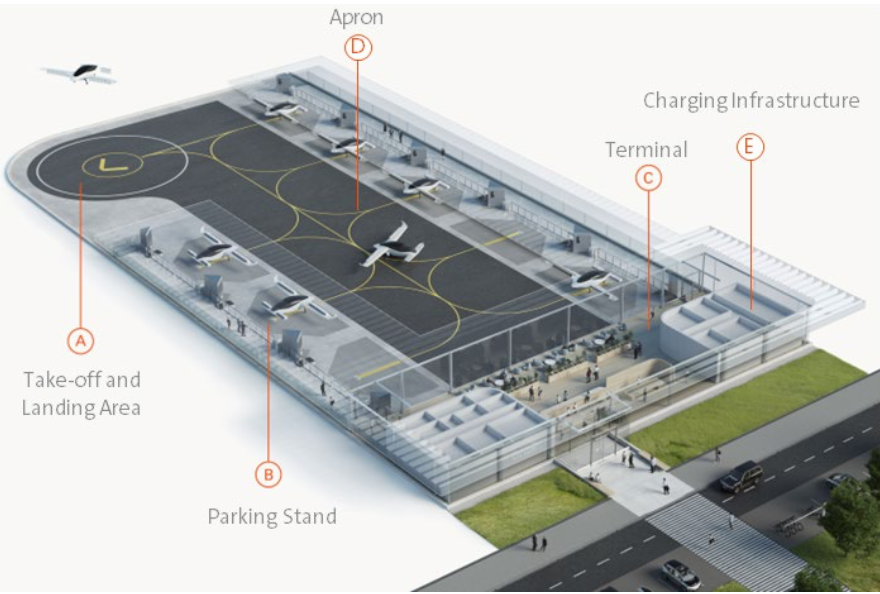
\includegraphics[width=0.7\linewidth]{figures/Market Analysis/Screenshot 2024-06-25 at 10.12.25.png}
        \caption{Lilium vertiport configuration \cite{rijksoverheid_vertiports,lilium2020designvertiports}}
        \label{fig:horizon_UAM}
    \end{figure}


\section{UK Air Mobility Consortium}
\label{sec:UKAM_Consortium}
As the geographical market segment for this project is projected to be London, the UK Air Mobility Consortium is considered to be of paramount importance.
More so, as the consortium accurately described their UAM Concept of Operations (CONOPS) for the London Environment \cite{UKAMC2022conops}, as well as being the main regulatory body of the UK’s UAM\@.
The Consortium consists of the UK's leading air traffic control provider; NATS, main airports; Heathrow and London City Airport, eVTOL manufacturers; Eve (Embraer), Vertical Aerospace and Volocopter, UAM developers; Atech (Embraer) and Harris Corporation, the leading vertiport provider; Skyports, and many more industry-leading partners.
Hence, adhering to the Consortium’s regulations and partnering up is of great interest to this project.
The earlier mentioned CONOPS does not only focus on the introduction of UAM, but the whole phase of development of UAM, eVTOLS, and additional challenges are considered. 
The Consortium strives to be ahead of the technology, thus competition, hence using a wide array of partners.
Therefore, the first step when, and even before, entering the market should be joining the UK UAM Consortium, as this project will significantly benefit from it.

\begin{figure}[H]
    \centering
    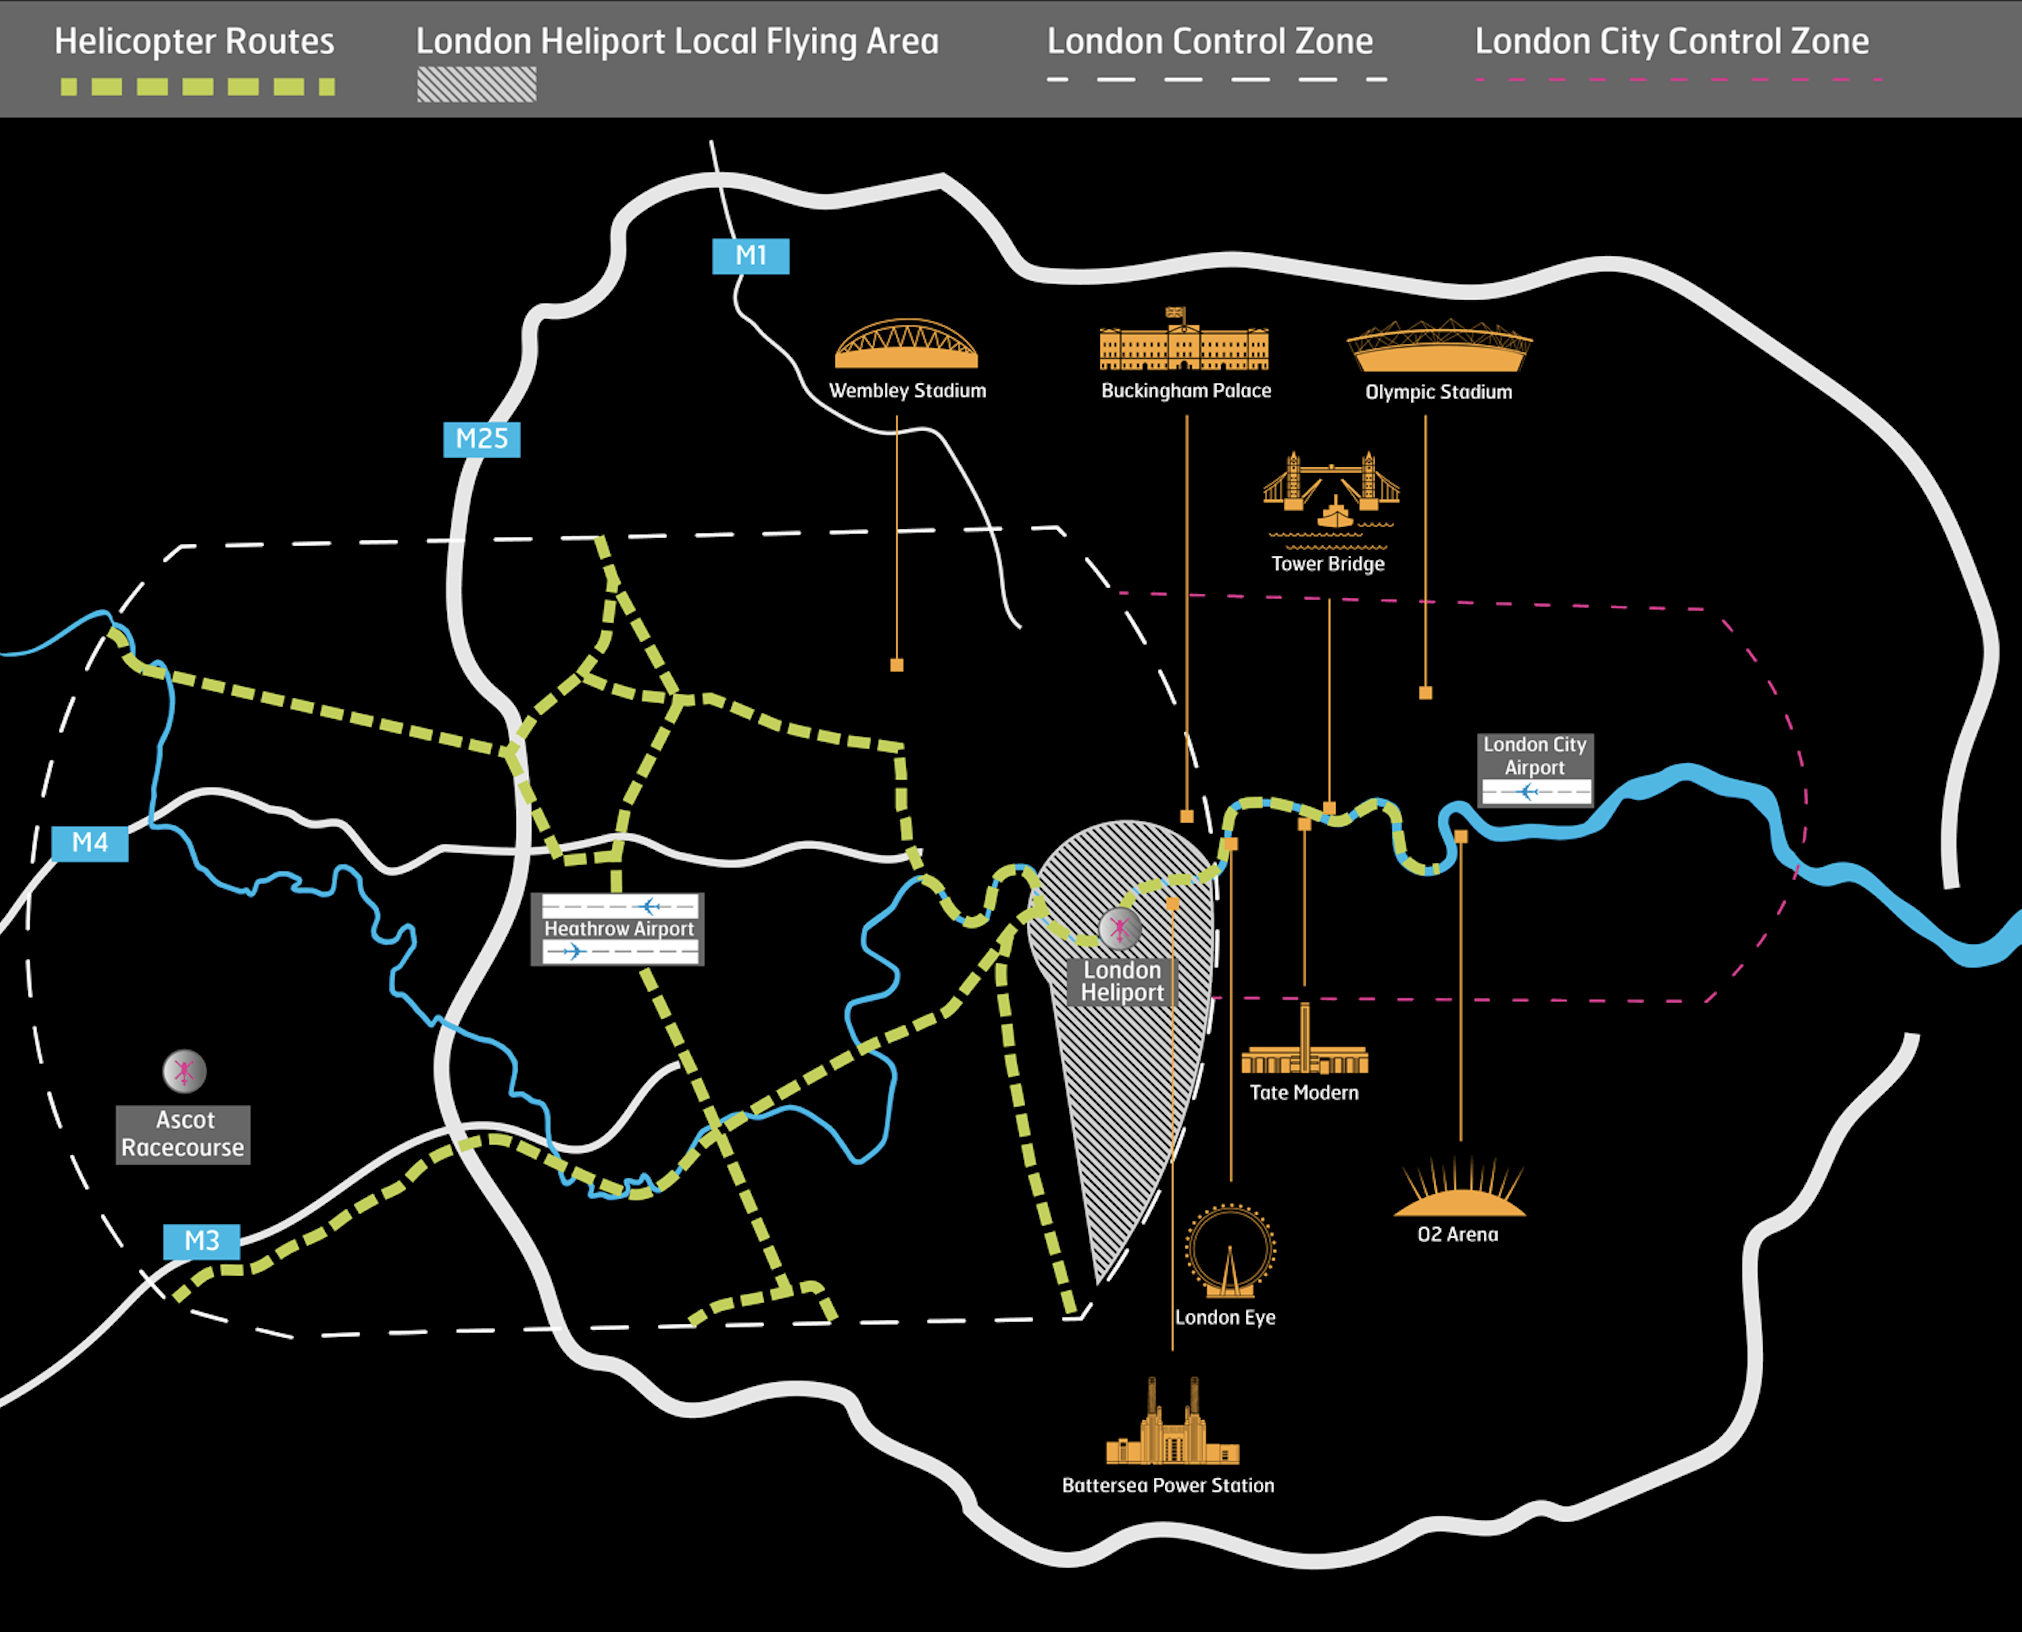
\includegraphics[width=0.6\linewidth]{figures/Market Analysis/NATS-heliroutes}
    \caption{London helicopter routes (NATS) \cite{UKAMC2022conops}}
    \label{fig:NATS_heliroutes}
\end{figure}


Besides the possibilities that the Consortium brings, it also provides the principal regulations regarding UAM, which is the main framework to adhere to.
Therefore, joining the Consortium would relieve the team of much work on certifying and adhering to the current laws.
The CONOPS already provides a pre-UAM defined landscape by performing tests with Skyports on a few London-based heliports, but also planning the first flights over the River Thames and highways, which will reduce the noise and privacy concerns of the public.
As the network of heliports is already established in the metropolitan area of London, which can be seen from \Cref{fig:NATS_heliroutes}, it will account for a fluent transition at the beginning of UAM integration.
Furthermore, the Consortium also has provided a UAM network possible around the River Thames in London's tightly packed city centre, mainly consisting of vertistops.
Both in the current and future flight paths, due to noise and privacy concerns, mainly the River Thames and highways are considered, as seen from the figure.

Therefore, the extensive CONOPS provided by the Consortium can be seen as the framework for the \textit{Swing eVTOL} and shows the importance of joining it.
Also, the active vertiport testbeds by Skyports, which have acquired two active heliports in London, are also available.
An interesting addition to the CONOPS would, however, be the integration of the OFV into London vertiports (\Cref{fig:OFV_London}), as this is one of the newest additions to UAM regulations, which is there to stay.
The adjacent operations and logistics are discussed in \Cref{ch:Operations_and_Logistics} for additional vertiport information.

\begin{minipage}{0.55\linewidth}
    \begin{figure}[H]
        \centering
        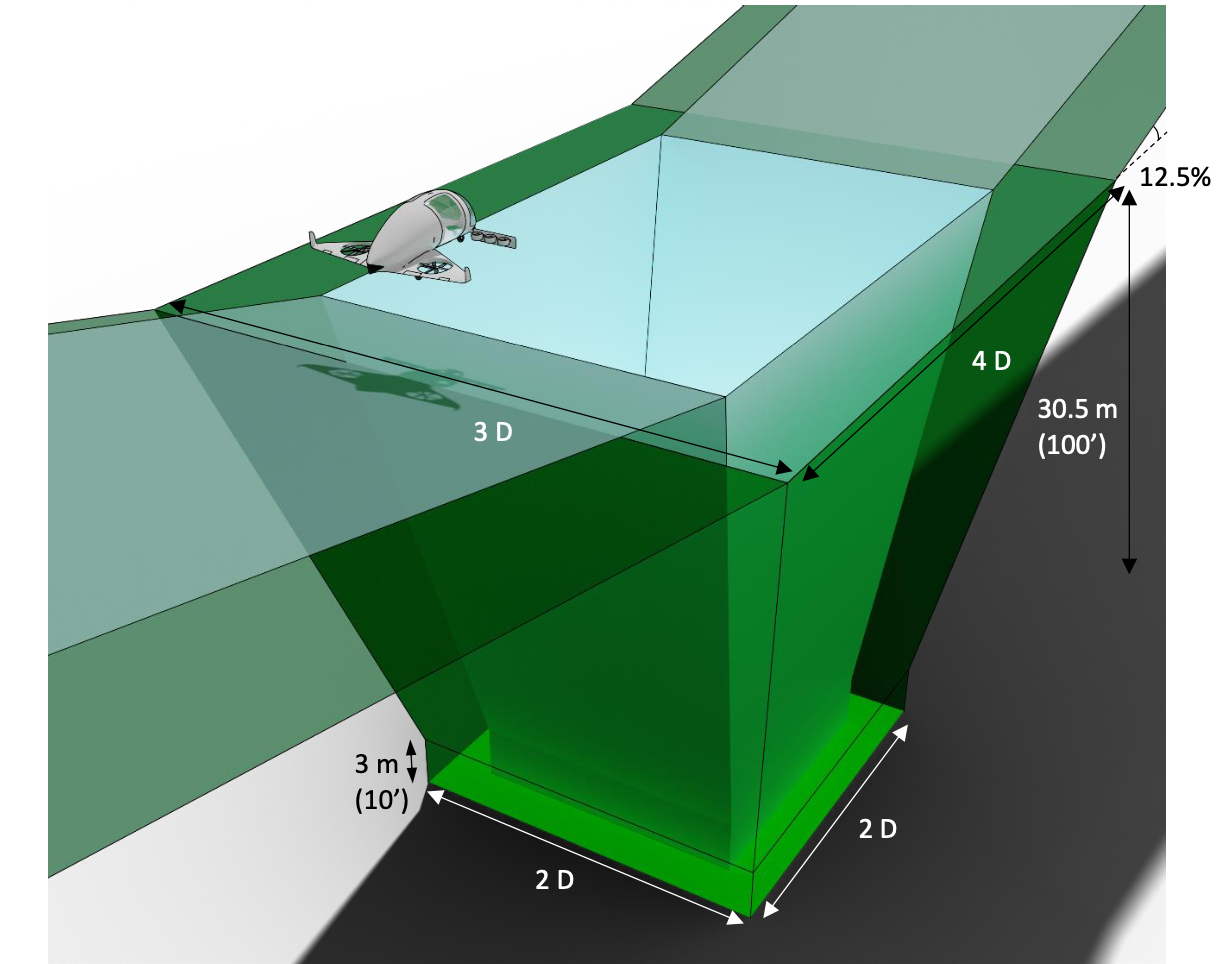
\includegraphics[width=.9\linewidth]{figures/Market Analysis/OFV_vertiport}
        \caption{EASA’s type 1 OFV \cite{easa2022vertiports}}
        \label{fig:OFV_vertiports}
    \end{figure}
\end{minipage}
\begin{minipage}{0.45\linewidth}
    \begin{figure}[H]
        \centering
        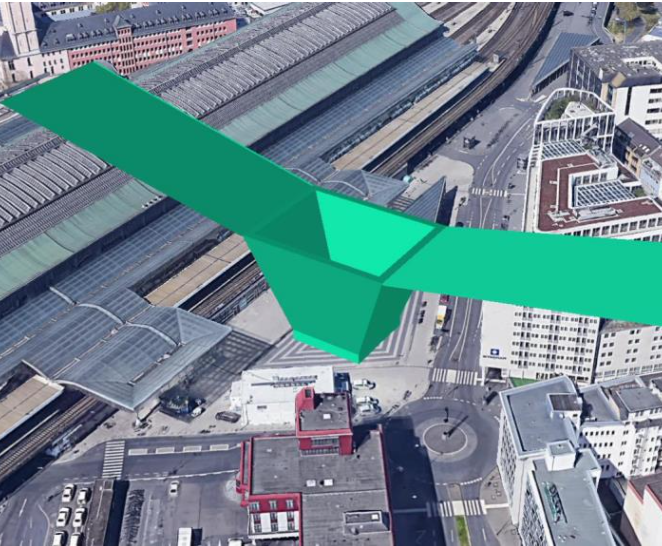
\includegraphics[width=0.9\linewidth]{figures/Market Analysis/OFV_application}
        \caption{OFV train station integration \cite{easa2022vertiports}}
        \label{fig:OFV_London}
    \end{figure}
\end{minipage}


\section{Competition Analysis}
\label{sec:Competition_Analysis}
As the exact market segmentation, infrastructure, and possible partnership have been established, it is helpful to analyse the competition to retrieve the main competitors.
Conducting the competition analysis also provides more explicit competitive advantages and eventual disadvantages, further identifying the market position of the \textit{Swing}.
As stated earlier, the UAM is still in their infancy, making it easier for companies to penetrate the market.
Although many configurations exist among the eVTOL UAM prospects, the ones in \Cref{tab:comp_specs} can all facilitate the air taxi industry.
However, as can be deduced from the table, the specifications, performances and prices differ significantly; hence, they should be compared to their close competition.
The same goes for the \textit{Swing eVTOL}; its main competitors should be identifiable from the table.

\begin{table}[H]
    \caption{Competition specifications \cite{evtol_aircraft_catalogue,rijksoverheid_vertiports}}
    \label{tab:comp_specs}
    \centering
    \resizebox{\textwidth}{!}{%
        \begin{tabular}{llllS[table-format=3]S[table-format=4]lS[table-format=3]S[table-format=1.2]}
            \toprule
            \textbf{Configuration} & \textbf{Manufacturer} & \textbf{Project}   & \textbf{Propulsion}        & \textbf{Ground} & \textbf{MTOW {[}kg{]}} & \textbf{Payload} & \textbf{Range} & \textbf{Price} \\
            & & & & \textbf{Footprint {[\unit{m^2}]}} & & \textbf{[\unit{pax}]} & \textbf{[\unit{km}]} & \textbf{[\unit{mil\$}]} \\ \midrule
            Multicopter            & Volocopter            & Volocity           & 18 rotors                  & 128           & 900                    & 1 + pilot                  & 65                   & 0.38             \\
            Multicopter            & eHang                 & EH216-S            & 16 rotors                  & 32          & 250                    & 2                  & 35                      & 0.3               \\
            Lift + Cruise          & Wisk                  & Cora               & 12 rotors + 1 pusher       & 70             & {-}                      & 2                  & 100                     & {-}                        \\
            Lift + Cruise          & Beta Technologies     & Alia               & 4 rotors + 1 pusher rotor  & 120                       & 3175                  & 4 + pilot               & 500                     & 4                 \\
            Lift + Cruise          & Volocopter            & VoloRegion         & 6 rotors + 2 ducted fans   & {-}                           & {-}                      & 4                  & 100                     & {-}                        \\
            Lift + Cruise          & Autoflight            & Prosperity I       & 13 rotors                  & 168            & 1500                    & 4                  & 250                     & 0.15              \\
            Vectored Thrust        & Embraer X             & EVE                & 8 rotors + 2 pusher rotors & 124           & 997                    & 4 + pilot               & 100                     & 2                 \\
            Vectored Thrust        & Airbus                & CityAirbus NextGen & 8 rotors                   & 182         & 1600                   & 3 + pilot                  & 80                      & {-}                        \\
            Vectored Thrust        & Lilium                & Lilium Jet         & 36 ducted fans             & 118           & 3175                  & 6 + pilot               & 250                     & 4                 \\
            Tiltrotor              & Sabrewing             & Rhaegal RG-1       & 4 ducted tiltrotors        & 248             & 4016                  & \qty{2454}{\kg}            & 185                    & {-}                        \\
            Tiltrotor              & Joby Aviation         & S4                 & 6 tiltrotors               & 76            & 2404                  & 4 + pilot        & 161                     & 1.3               \\
            Tiltrotor              & Vertical Aerospace    & VX4                & 4 tilt + 4 stowable rotors & 195          & {-}                      & 4 + pilot               & 161                     & 4                 \\
            Tiltrotor              & Archer Aviation       & Midnight           & 12 rotors (6 tiltrotors)   & 88                     & 3175                  & 4 + pilot               & 80                   & 5       \\ \midrule
            \textbf{Transwing}     & \textbf{DSE Group 1}  & \bfemph{Swing eVTOL}     & \textbf{6 rotors}          & \textbf{32} & \textbf{1643} & \textbf{4} & \textbf{250} & \textbf{2.2} \\
            \bottomrule
        \end{tabular}
    }
\end{table}


When looking at \Cref{tab:comp_specs}, the most apparent distinction between vehicles is their configuration, thus the way of realising UAM.
The multicopters, through their drone-like flight, are very stable and flexible in their low ground footprint; however, they lack the range for interurban travel.
So-called \enquote*{Lift+Cruise} configurations conclude separate lift rotors with cruise, or better-known pusher, rotors.
The range gets remarkably better due to their wing designs; however, they do not have a low ground footprint suitable for population-dense areas.
The same goes for the vectored thrust and tiltrotors configurations, although very innovative, it does not account for the needed low ground footprint.
Hence, the transwing configuration perfectly tackles the problem of the competition, delivering the best of both worlds.
Moreover, the prices of the last two configurations are considerably higher, while those of the multicopter are the lowest on average.

\begin{minipage}{0.5\linewidth}
    \begin{figure}[H]
        \centering
        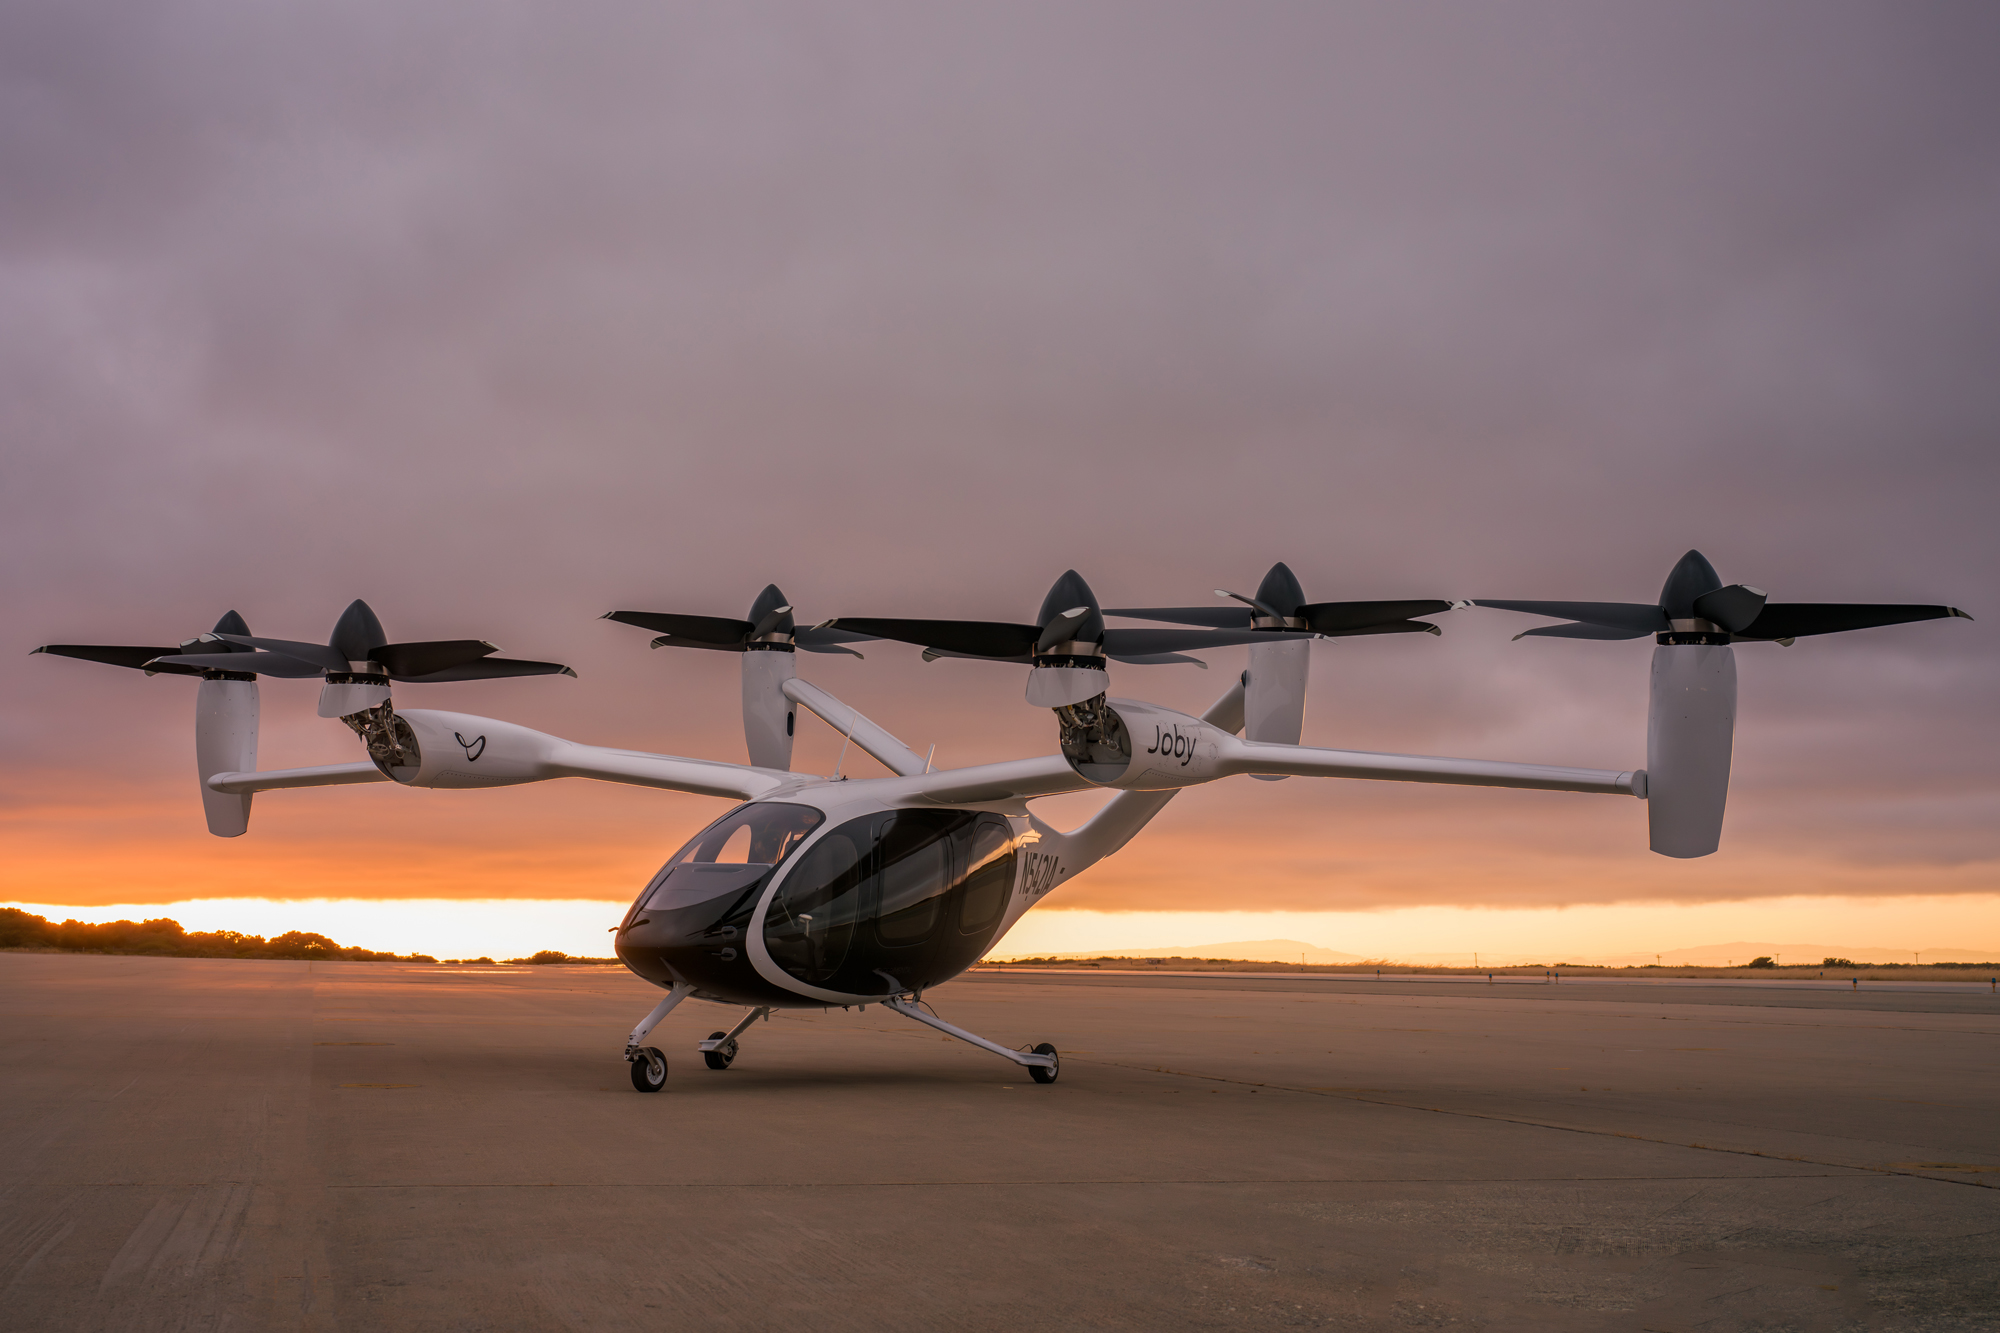
\includegraphics[width=.95\linewidth]{figures/Market Analysis/Joby-Aviation-production-prototoype-June-28-2023}
        \caption{Joby S4 \cite{evtol_aircraft_catalogue}}
        \label{fig:Joby_s4}
    \end{figure}
\end{minipage}
\begin{minipage}{0.5\linewidth}
    \begin{figure}[H]
        \centering
        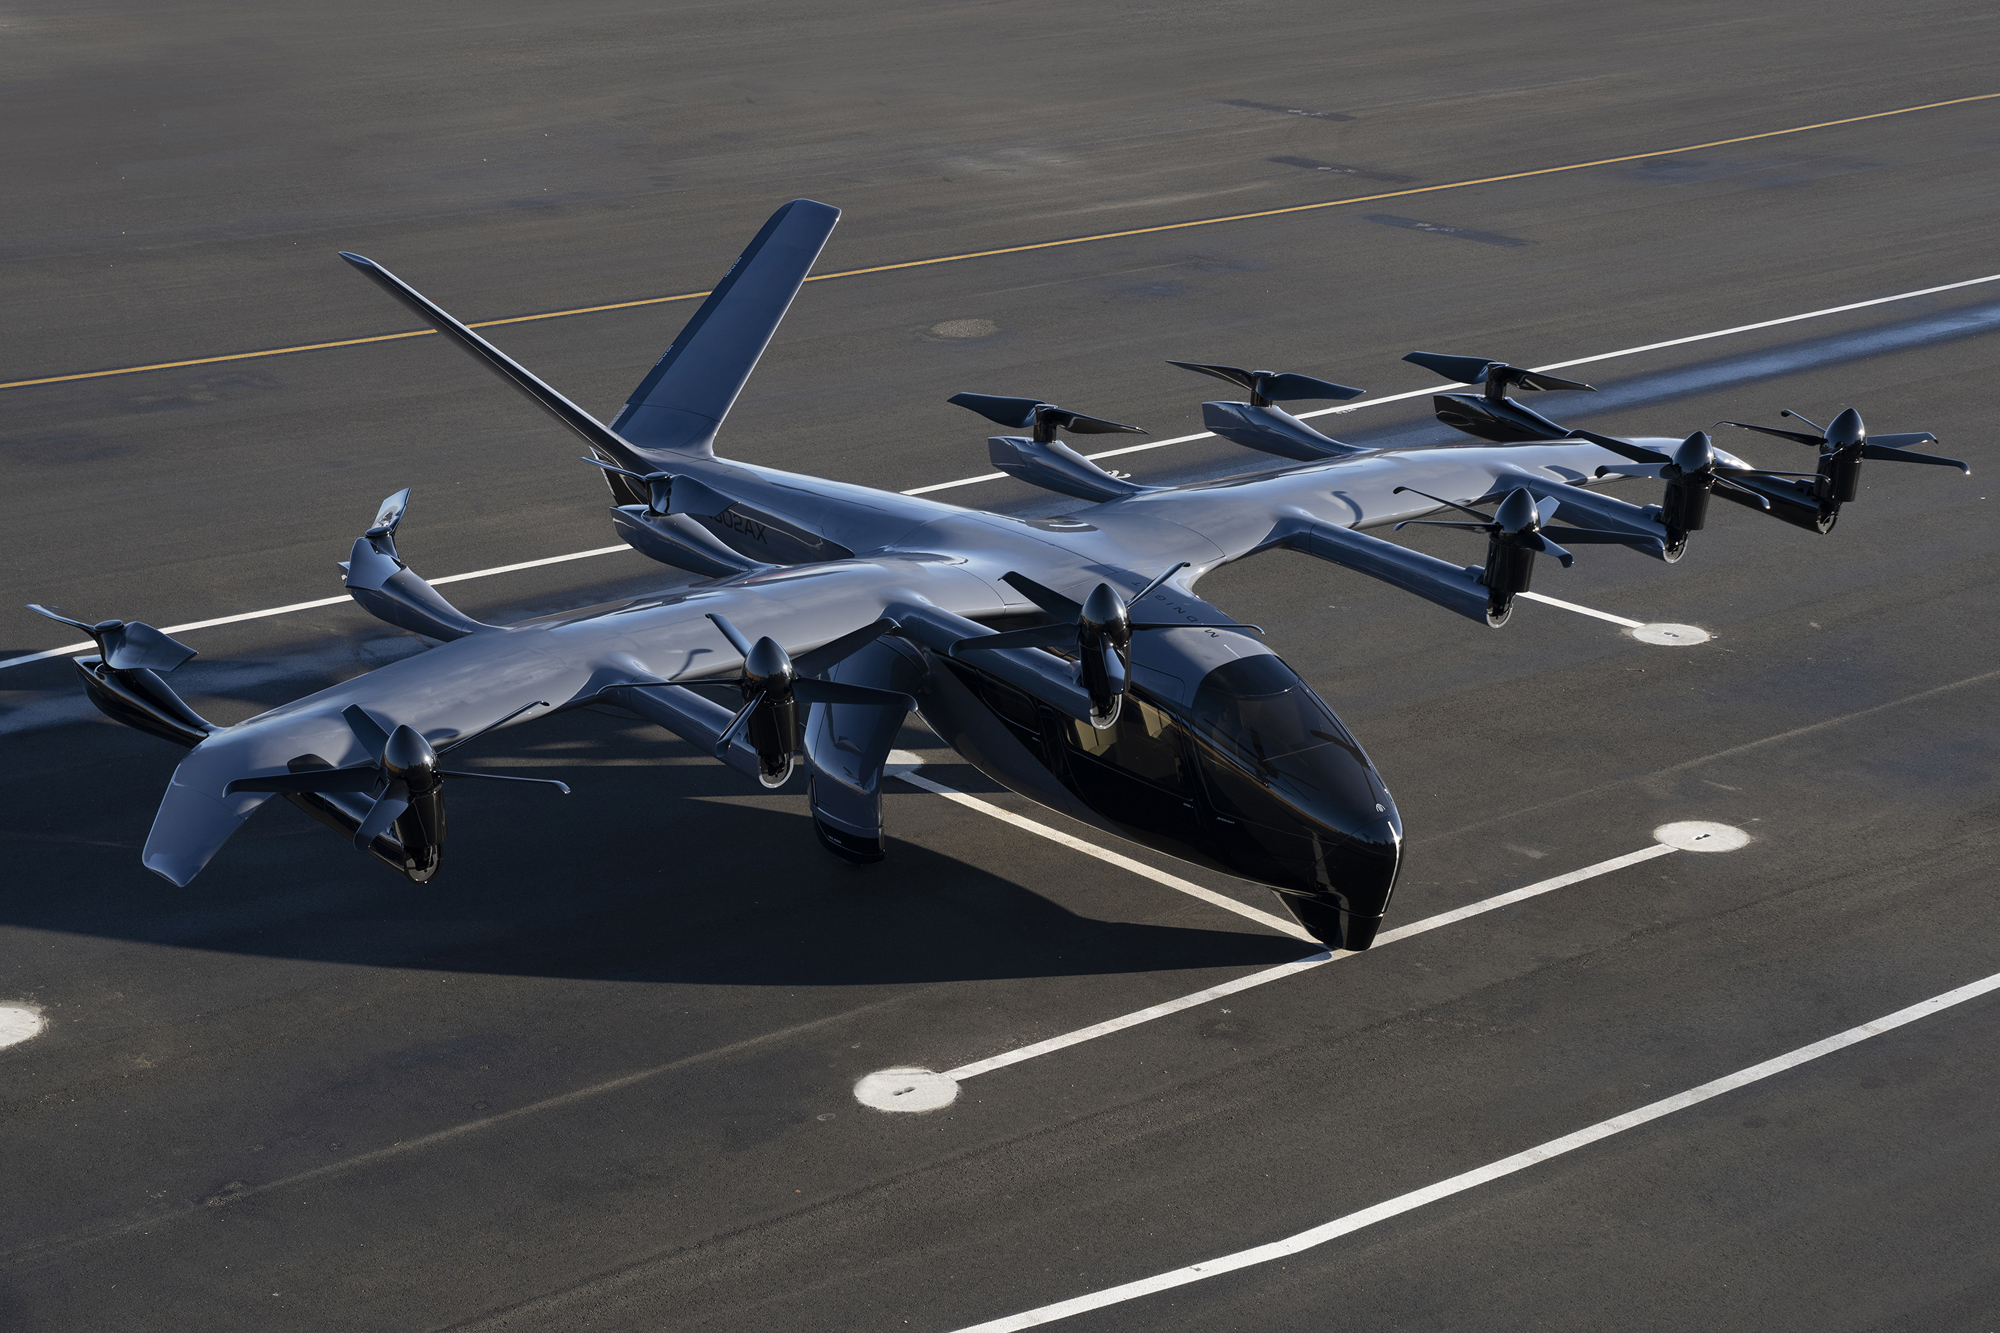
\includegraphics[width=.95\linewidth]{figures/Market Analysis/Archer_Midnight_top_view}
        \caption{Archer Midnight \cite{evtol_aircraft_catalogue}}
        \label{fig:Archer_midnight}
    \end{figure}
\end{minipage}

\subsection{Main Competitors}
The Joby S4 (\Cref{fig:Joby_s4}) particularly stand out due to its relatively small wingspan in combination with a great range of \qty{161}{km}.
Also, as previously discussed, it is considered one of the quietest eVTOLs on the market, with a noise production of 65 dBA at 330 feet (\qty{100}{m}) in VTOL configuration, and only 45 dBA at 1640 feet (\qty{500}{m}) in cruise configuration \cite{nasaxjoby2022acoustic,joby2022decibel}.
It is a competitor to be closely monitored, as it is the most promising in-production prospect.
Although the \textit{Swing eVTOL} still outperforms the Joby S4 on the ground footprint aspect, which may turn out to be the most constraining.
Furthermore, the Archer Midnight (\Cref{fig:Archer_midnight}) has already started production of \num{2300} units a year and secured a 1-billion-dollar order from United Airlines.
It even got approval from the FAA for commercial flight and thus is realistically the main competitor on the market.
However, the eVTOL comes with a relatively high price tag of 5 million USD with a limited range of 32 to 80 km and a comparatively high wingspan.
Therefore, the \textit{Swing} outperforms the range, ground footprint, and price, making it a more favourable prospect.

\subsection{Mission SWOT Analysis}
As a last measure, a mission Strengths Weaknesses Opportunities and Threats (SWOT) analysis provides the competitive edge of the \textit{Swing eVTOL}.
It is essential to note the positives; however, identifying the weaknesses and threats of the mission is of even greater interest.
The final mission SWOT analysis is established in \Cref{fig:swot-analysis}.

\begin{figure}[H]
    \centering
    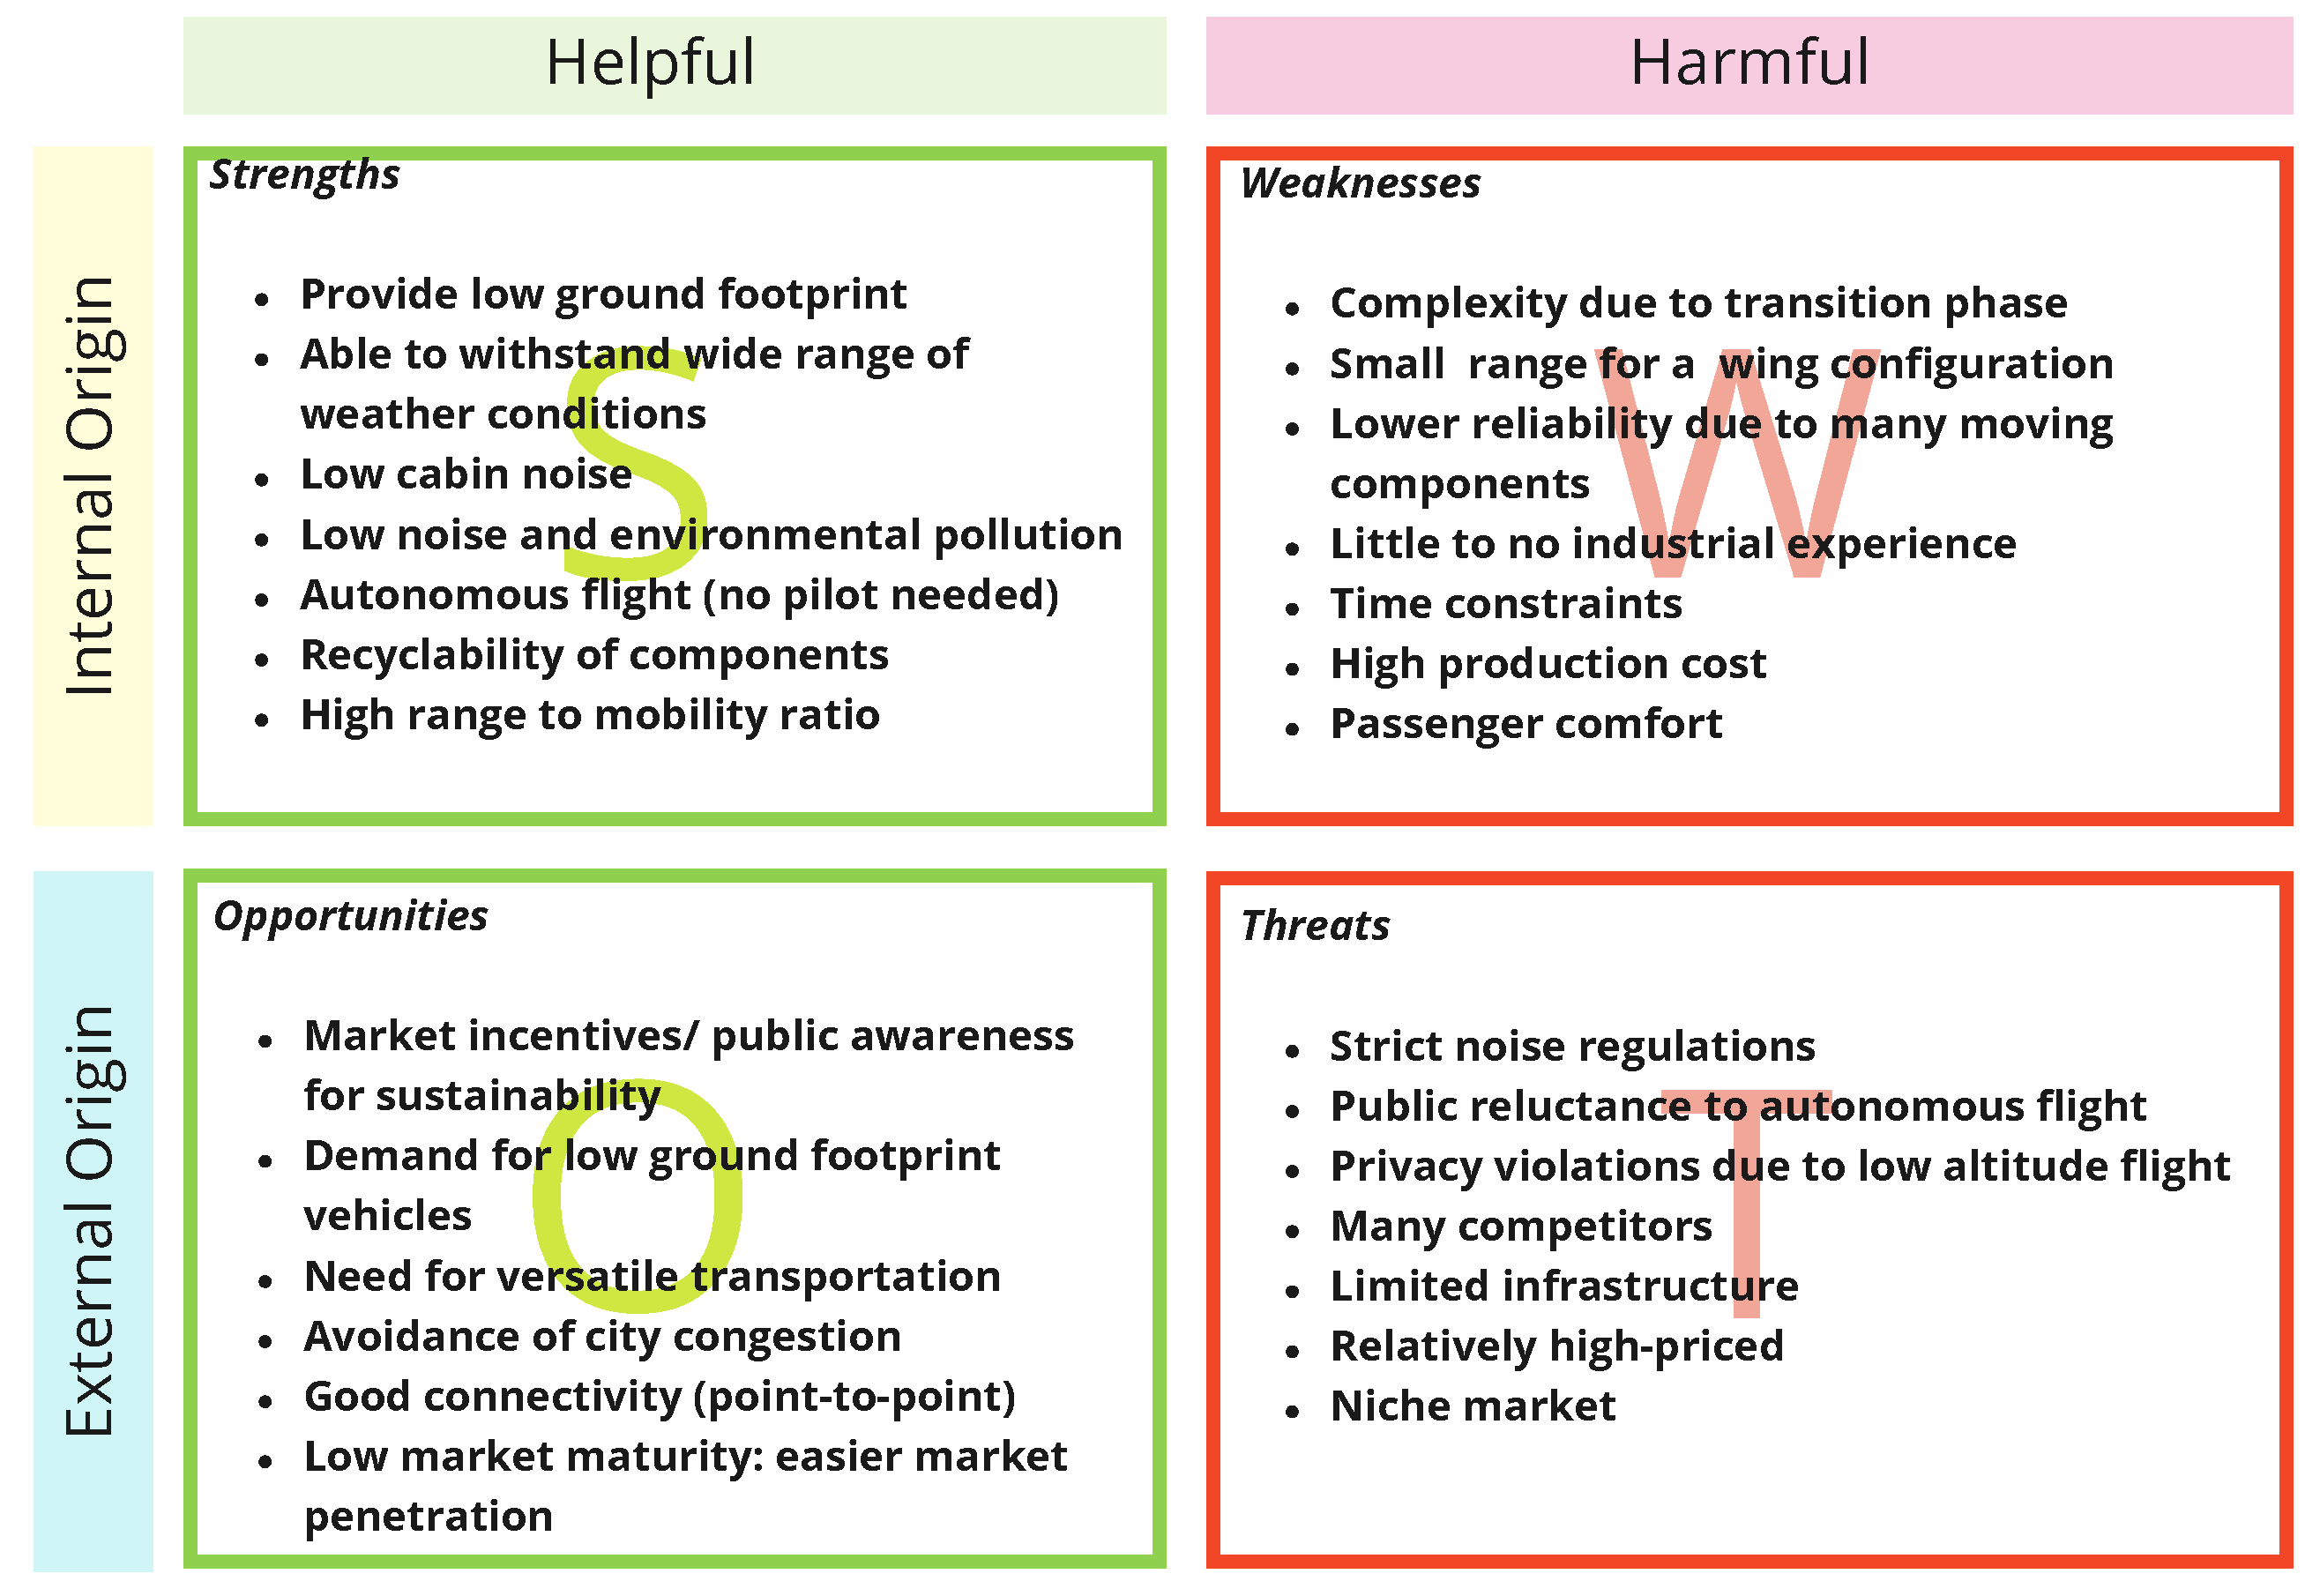
\includegraphics[width=0.7\linewidth]{figures/Market Analysis/Copy SWOT Analysis}
    \caption{SWOT Analysis}
    \label{fig:swot-analysis}
\end{figure}

\subsection{Differentiation Factor}
\label{sec:differentiation_factor}
Concluding the market analysis, the differentiation factors of the \textit{Swing eVTOL} ought to be discussed.
The London metropolitan area is the perfect introductory market segmentation, facilitating all use cases and infrastructure, and a strong UAM partner in the UK Air Mobility Consortium.
Moreover, the competition analysis showed the unique selling point of having a greater range while still accounting for a low ground footprint of four parking spots.
This can even realise the heavily sought after last-mile transportation while still accommodating intercity flights.
\Cref{tab:possible_usecases} perfectly shows the unique place of the \textit{Swing eVTOL} in the UAM market, being able to capitalise on all the market segments.
Moreover, the further competitive edge on energy consumption and cost will be discussed in \Cref{sec:energyconsumption}.
In the long term, certifications with ground regulatory bodies, instead of only air traffic, could be of great potential.
The four parking spots truly bring a totally new dynamic within the UAM market.

\begin{table}[H]
    \centering
    \caption{Differentiation of \textit{Swing eVTOL} in market segments}
    \label{tab:possible_usecases}
    \resizebox{0.7\textwidth}{!}{%
    \begin{tabular}{l|c|c|c|c}
        \toprule
        \textbf{eVTOL}       & \textbf{Air Taxi }    &  \textbf{Airport Shuttle} &\textbf{Intercity Flights}    &   \textbf{Last-mile transport}     \\ \midrule
        \textit{Swing}        &X& X & X & X             \\
        Joby S4    &X& X & X & -             \\
        Archer Midnight   &X& X & - & -             \\
        EHang 216-S    &X& - & - & X             \\\bottomrule
    \end{tabular}%
    }
\end{table}
